\section{Program description}

\begin{figure}[h!]
	\centering
	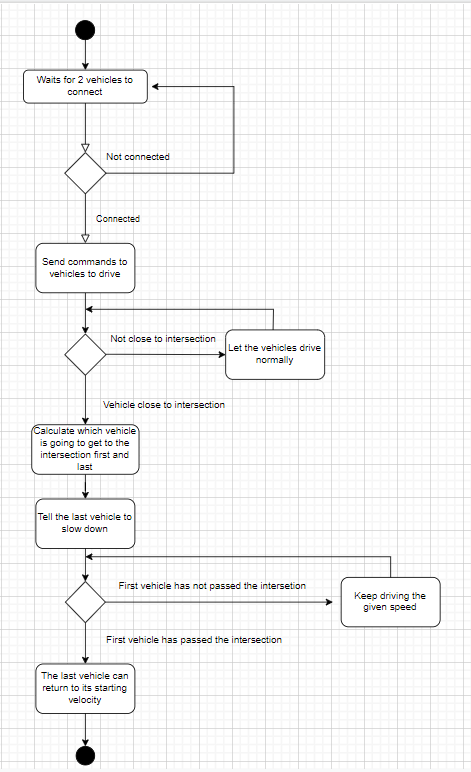
\includegraphics[width=1\linewidth]{figures/Flow_diagram_server}
	\caption[Flow diagram server]{Flow diagram for the server. This diagram specificly shows the flow of the demo}
	\label{fig:diagramserver}
\end{figure}

The program is an IoT-system were vehicles can communicate with eachother through a server. It constists of a server which has the responsibility for the calculations and decision making, and a client which are the vehicles. The function of the program is to increase traffic flow and prevent traffic congestion. As of now the program can be used in an intersection with two vehicles, but can be scaled to include more vehicles. Here is a diagram that describes the flow of our server in the demonstration:



